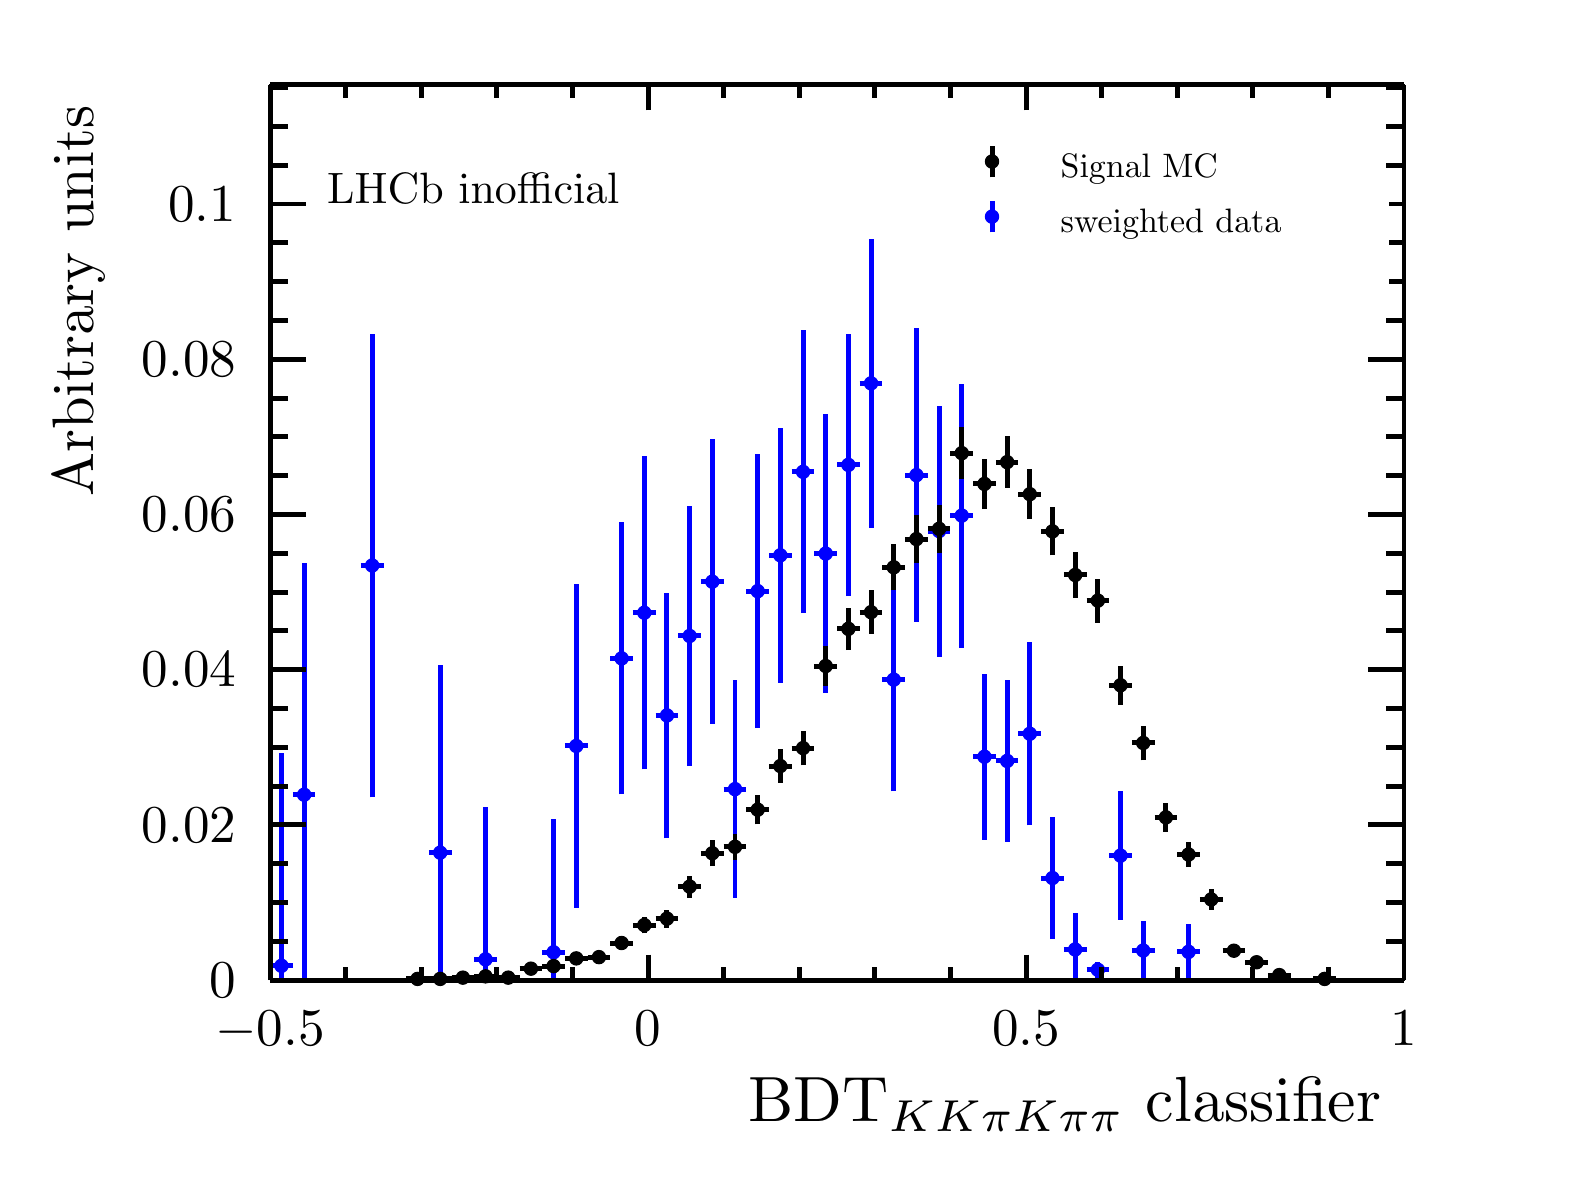
\begin{tikzpicture}
\pgfdeclareplotmark{cross} {
\pgfpathmoveto{\pgfpoint{-0.3\pgfplotmarksize}{\pgfplotmarksize}}
\pgfpathlineto{\pgfpoint{+0.3\pgfplotmarksize}{\pgfplotmarksize}}
\pgfpathlineto{\pgfpoint{+0.3\pgfplotmarksize}{0.3\pgfplotmarksize}}
\pgfpathlineto{\pgfpoint{+1\pgfplotmarksize}{0.3\pgfplotmarksize}}
\pgfpathlineto{\pgfpoint{+1\pgfplotmarksize}{-0.3\pgfplotmarksize}}
\pgfpathlineto{\pgfpoint{+0.3\pgfplotmarksize}{-0.3\pgfplotmarksize}}
\pgfpathlineto{\pgfpoint{+0.3\pgfplotmarksize}{-1.\pgfplotmarksize}}
\pgfpathlineto{\pgfpoint{-0.3\pgfplotmarksize}{-1.\pgfplotmarksize}}
\pgfpathlineto{\pgfpoint{-0.3\pgfplotmarksize}{-0.3\pgfplotmarksize}}
\pgfpathlineto{\pgfpoint{-1.\pgfplotmarksize}{-0.3\pgfplotmarksize}}
\pgfpathlineto{\pgfpoint{-1.\pgfplotmarksize}{0.3\pgfplotmarksize}}
\pgfpathlineto{\pgfpoint{-0.3\pgfplotmarksize}{0.3\pgfplotmarksize}}
\pgfpathclose
\pgfusepathqstroke
}
\pgfdeclareplotmark{cross*} {
\pgfpathmoveto{\pgfpoint{-0.3\pgfplotmarksize}{\pgfplotmarksize}}
\pgfpathlineto{\pgfpoint{+0.3\pgfplotmarksize}{\pgfplotmarksize}}
\pgfpathlineto{\pgfpoint{+0.3\pgfplotmarksize}{0.3\pgfplotmarksize}}
\pgfpathlineto{\pgfpoint{+1\pgfplotmarksize}{0.3\pgfplotmarksize}}
\pgfpathlineto{\pgfpoint{+1\pgfplotmarksize}{-0.3\pgfplotmarksize}}
\pgfpathlineto{\pgfpoint{+0.3\pgfplotmarksize}{-0.3\pgfplotmarksize}}
\pgfpathlineto{\pgfpoint{+0.3\pgfplotmarksize}{-1.\pgfplotmarksize}}
\pgfpathlineto{\pgfpoint{-0.3\pgfplotmarksize}{-1.\pgfplotmarksize}}
\pgfpathlineto{\pgfpoint{-0.3\pgfplotmarksize}{-0.3\pgfplotmarksize}}
\pgfpathlineto{\pgfpoint{-1.\pgfplotmarksize}{-0.3\pgfplotmarksize}}
\pgfpathlineto{\pgfpoint{-1.\pgfplotmarksize}{0.3\pgfplotmarksize}}
\pgfpathlineto{\pgfpoint{-0.3\pgfplotmarksize}{0.3\pgfplotmarksize}}
\pgfpathclose
\pgfusepathqfillstroke
}
\pgfdeclareplotmark{newstar} {
\pgfpathmoveto{\pgfqpoint{0pt}{\pgfplotmarksize}}
\pgfpathlineto{\pgfqpointpolar{44}{0.5\pgfplotmarksize}}
\pgfpathlineto{\pgfqpointpolar{18}{\pgfplotmarksize}}
\pgfpathlineto{\pgfqpointpolar{-20}{0.5\pgfplotmarksize}}
\pgfpathlineto{\pgfqpointpolar{-54}{\pgfplotmarksize}}
\pgfpathlineto{\pgfqpointpolar{-90}{0.5\pgfplotmarksize}}
\pgfpathlineto{\pgfqpointpolar{234}{\pgfplotmarksize}}
\pgfpathlineto{\pgfqpointpolar{198}{0.5\pgfplotmarksize}}
\pgfpathlineto{\pgfqpointpolar{162}{\pgfplotmarksize}}
\pgfpathlineto{\pgfqpointpolar{134}{0.5\pgfplotmarksize}}
\pgfpathclose
\pgfusepathqstroke
}
\pgfdeclareplotmark{newstar*} {
\pgfpathmoveto{\pgfqpoint{0pt}{\pgfplotmarksize}}
\pgfpathlineto{\pgfqpointpolar{44}{0.5\pgfplotmarksize}}
\pgfpathlineto{\pgfqpointpolar{18}{\pgfplotmarksize}}
\pgfpathlineto{\pgfqpointpolar{-20}{0.5\pgfplotmarksize}}
\pgfpathlineto{\pgfqpointpolar{-54}{\pgfplotmarksize}}
\pgfpathlineto{\pgfqpointpolar{-90}{0.5\pgfplotmarksize}}
\pgfpathlineto{\pgfqpointpolar{234}{\pgfplotmarksize}}
\pgfpathlineto{\pgfqpointpolar{198}{0.5\pgfplotmarksize}}
\pgfpathlineto{\pgfqpointpolar{162}{\pgfplotmarksize}}
\pgfpathlineto{\pgfqpointpolar{134}{0.5\pgfplotmarksize}}
\pgfpathclose
\pgfusepathqfillstroke
}
\definecolor{c}{rgb}{1,1,1};
\draw [color=c, fill=c] (0.4,0) rectangle (19.6,14.393);
\draw [color=c, fill=c] (3.472,2.30288) rectangle (17.872,13.6733);
\definecolor{c}{rgb}{0,0,0};
\draw [c,line width=0.9] (3.472,2.30288) -- (3.472,13.6733) -- (17.872,13.6733) -- (17.872,2.30288) -- (3.472,2.30288);
\definecolor{c}{rgb}{1,1,1};
\draw [color=c, fill=c] (3.472,2.30288) rectangle (17.872,13.6733);
\definecolor{c}{rgb}{0,0,0};
\draw [c,line width=0.9] (3.472,2.30288) -- (3.472,13.6733) -- (17.872,13.6733) -- (17.872,2.30288) -- (3.472,2.30288);
\definecolor{c}{rgb}{0,0,1};
\draw [c,line width=1.8] (3.616,2.30288) -- (3.616,2.43551);
\draw [c,line width=1.8] (3.616,2.53576) -- (3.616,5.19284);
\draw [c,line width=1.8] (3.472,2.48564) -- (3.56587,2.48564);
\draw [c,line width=1.8] (3.66613,2.48564) -- (3.76,2.48564);
\foreach \P in {(3.616,2.48564)}{\draw[mark options={color=c,fill=c},mark size=2.402402pt,mark=*] plot coordinates {\P};}
\draw [c,line width=1.8] (3.904,2.30288) -- (3.904,4.60855);
\draw [c,line width=1.8] (3.904,4.7088) -- (3.904,7.59555);
\draw [c,line width=1.8] (3.76,4.65867) -- (3.85387,4.65867);
\draw [c,line width=1.8] (3.95413,4.65867) -- (4.048,4.65867);
\foreach \P in {(3.904,4.65867)}{\draw[mark options={color=c,fill=c},mark size=2.402402pt,mark=*] plot coordinates {\P};}
\draw [c,line width=1.8] (4.768,4.62392) -- (4.768,7.51958);
\draw [c,line width=1.8] (4.768,7.61983) -- (4.768,10.5155);
\draw [c,line width=1.8] (4.624,7.5697) -- (4.71787,7.5697);
\draw [c,line width=1.8] (4.81813,7.5697) -- (4.912,7.5697);
\foreach \P in {(4.768,7.5697)}{\draw[mark options={color=c,fill=c},mark size=2.402402pt,mark=*] plot coordinates {\P};}
\draw [c,line width=1.8] (5.632,2.30288) -- (5.632,3.87272);
\draw [c,line width=1.8] (5.632,3.97297) -- (5.632,6.30188);
\draw [c,line width=1.8] (5.488,3.92285) -- (5.58187,3.92285);
\draw [c,line width=1.8] (5.68213,3.92285) -- (5.776,3.92285);
\foreach \P in {(5.632,3.92285)}{\draw[mark options={color=c,fill=c},mark size=2.402402pt,mark=*] plot coordinates {\P};}
\draw [c,line width=1.8] (6.208,2.30288) -- (6.208,2.51738);
\draw [c,line width=1.8] (6.208,2.61764) -- (6.208,4.50221);
\draw [c,line width=1.8] (6.064,2.56751) -- (6.15787,2.56751);
\draw [c,line width=1.8] (6.25813,2.56751) -- (6.352,2.56751);
\foreach \P in {(6.208,2.56751)}{\draw[mark options={color=c,fill=c},mark size=2.402402pt,mark=*] plot coordinates {\P};}
\draw [c,line width=1.8] (7.072,2.30288) -- (7.072,2.60748);
\draw [c,line width=1.8] (7.072,2.70773) -- (7.072,4.35119);
\draw [c,line width=1.8] (6.928,2.6576) -- (7.02187,2.6576);
\draw [c,line width=1.8] (7.12213,2.6576) -- (7.216,2.6576);
\foreach \P in {(7.072,2.6576)}{\draw[mark options={color=c,fill=c},mark size=2.402402pt,mark=*] plot coordinates {\P};}
\draw [c,line width=1.8] (7.36,3.22389) -- (7.36,5.22759);
\draw [c,line width=1.8] (7.36,5.32784) -- (7.36,7.33153);
\draw [c,line width=1.8] (7.216,5.27771) -- (7.30987,5.27771);
\draw [c,line width=1.8] (7.41013,5.27771) -- (7.504,5.27771);
\foreach \P in {(7.36,5.27771)}{\draw[mark options={color=c,fill=c},mark size=2.402402pt,mark=*] plot coordinates {\P};}
\draw [c,line width=1.8] (7.936,4.66209) -- (7.936,6.3401);
\draw [c,line width=1.8] (7.936,6.44035) -- (7.936,8.11836);
\draw [c,line width=1.8] (7.792,6.39023) -- (7.88587,6.39023);
\draw [c,line width=1.8] (7.98613,6.39023) -- (8.08,6.39023);
\foreach \P in {(7.936,6.39023)}{\draw[mark options={color=c,fill=c},mark size=2.402402pt,mark=*] plot coordinates {\P};}
\draw [c,line width=1.8] (8.224,4.98012) -- (8.224,6.91956);
\draw [c,line width=1.8] (8.224,7.01981) -- (8.224,8.95925);
\draw [c,line width=1.8] (8.08,6.96969) -- (8.17387,6.96969);
\draw [c,line width=1.8] (8.27413,6.96969) -- (8.368,6.96969);
\foreach \P in {(8.224,6.96969)}{\draw[mark options={color=c,fill=c},mark size=2.402402pt,mark=*] plot coordinates {\P};}
\draw [c,line width=1.8] (8.512,4.10466) -- (8.512,5.61531);
\draw [c,line width=1.8] (8.512,5.71556) -- (8.512,7.22622);
\draw [c,line width=1.8] (8.368,5.66544) -- (8.46187,5.66544);
\draw [c,line width=1.8] (8.56213,5.66544) -- (8.656,5.66544);
\foreach \P in {(8.512,5.66544)}{\draw[mark options={color=c,fill=c},mark size=2.402402pt,mark=*] plot coordinates {\P};}
\draw [c,line width=1.8] (8.8,5.02088) -- (8.8,6.62468);
\draw [c,line width=1.8] (8.8,6.72494) -- (8.8,8.32874);
\draw [c,line width=1.8] (8.656,6.67481) -- (8.74988,6.67481);
\draw [c,line width=1.8] (8.85013,6.67481) -- (8.944,6.67481);
\foreach \P in {(8.8,6.67481)}{\draw[mark options={color=c,fill=c},mark size=2.402402pt,mark=*] plot coordinates {\P};}
\draw [c,line width=1.8] (9.088,5.55668) -- (9.088,7.31396);
\draw [c,line width=1.8] (9.088,7.41421) -- (9.088,9.17148);
\draw [c,line width=1.8] (8.944,7.36408) -- (9.03787,7.36408);
\draw [c,line width=1.8] (9.13813,7.36408) -- (9.232,7.36408);
\foreach \P in {(9.088,7.36408)}{\draw[mark options={color=c,fill=c},mark size=2.402402pt,mark=*] plot coordinates {\P};}
\draw [c,line width=1.8] (9.376,3.34812) -- (9.376,4.67979);
\draw [c,line width=1.8] (9.376,4.78004) -- (9.376,6.11171);
\draw [c,line width=1.8] (9.232,4.72991) -- (9.32587,4.72991);
\draw [c,line width=1.8] (9.42613,4.72991) -- (9.52,4.72991);
\foreach \P in {(9.376,4.72991)}{\draw[mark options={color=c,fill=c},mark size=2.402402pt,mark=*] plot coordinates {\P};}
\draw [c,line width=1.8] (9.664,5.50558) -- (9.664,7.19387);
\draw [c,line width=1.8] (9.664,7.29412) -- (9.664,8.98242);
\draw [c,line width=1.8] (9.52,7.244) -- (9.61387,7.244);
\draw [c,line width=1.8] (9.71413,7.244) -- (9.808,7.244);
\foreach \P in {(9.664,7.244)}{\draw[mark options={color=c,fill=c},mark size=2.402402pt,mark=*] plot coordinates {\P};}
\draw [c,line width=1.8] (9.952,6.07966) -- (9.952,7.64889);
\draw [c,line width=1.8] (9.952,7.74914) -- (9.952,9.31837);
\draw [c,line width=1.8] (9.808,7.69902) -- (9.90187,7.69902);
\draw [c,line width=1.8] (10.0021,7.69902) -- (10.096,7.69902);
\foreach \P in {(9.952,7.69902)}{\draw[mark options={color=c,fill=c},mark size=2.402402pt,mark=*] plot coordinates {\P};}
\draw [c,line width=1.8] (10.24,6.9633) -- (10.24,8.70897);
\draw [c,line width=1.8] (10.24,8.80922) -- (10.24,10.5549);
\draw [c,line width=1.8] (10.096,8.75909) -- (10.1899,8.75909);
\draw [c,line width=1.8] (10.2901,8.75909) -- (10.384,8.75909);
\foreach \P in {(10.24,8.75909)}{\draw[mark options={color=c,fill=c},mark size=2.402402pt,mark=*] plot coordinates {\P};}
\draw [c,line width=1.8] (10.528,5.95312) -- (10.528,7.67082);
\draw [c,line width=1.8] (10.528,7.77107) -- (10.528,9.48876);
\draw [c,line width=1.8] (10.384,7.72094) -- (10.4779,7.72094);
\draw [c,line width=1.8] (10.5781,7.72094) -- (10.672,7.72094);
\foreach \P in {(10.528,7.72094)}{\draw[mark options={color=c,fill=c},mark size=2.402402pt,mark=*] plot coordinates {\P};}
\draw [c,line width=1.8] (10.816,7.1796) -- (10.816,8.79733);
\draw [c,line width=1.8] (10.816,8.89758) -- (10.816,10.5153);
\draw [c,line width=1.8] (10.672,8.84745) -- (10.7659,8.84745);
\draw [c,line width=1.8] (10.8661,8.84745) -- (10.96,8.84745);
\foreach \P in {(10.816,8.84745)}{\draw[mark options={color=c,fill=c},mark size=2.402402pt,mark=*] plot coordinates {\P};}
\draw [c,line width=1.8] (11.104,8.04578) -- (11.104,9.83306);
\draw [c,line width=1.8] (11.104,9.93331) -- (11.104,11.7206);
\draw [c,line width=1.8] (10.96,9.88318) -- (11.0539,9.88318);
\draw [c,line width=1.8] (11.1541,9.88318) -- (11.248,9.88318);
\foreach \P in {(11.104,9.88318)}{\draw[mark options={color=c,fill=c},mark size=2.402402pt,mark=*] plot coordinates {\P};}
\draw [c,line width=1.8] (11.392,4.70152) -- (11.392,6.07005);
\draw [c,line width=1.8] (11.392,6.1703) -- (11.392,7.53883);
\draw [c,line width=1.8] (11.248,6.12017) -- (11.3419,6.12017);
\draw [c,line width=1.8] (11.4421,6.12017) -- (11.536,6.12017);
\foreach \P in {(11.392,6.12017)}{\draw[mark options={color=c,fill=c},mark size=2.402402pt,mark=*] plot coordinates {\P};}
\draw [c,line width=1.8] (11.68,6.85213) -- (11.68,8.66706);
\draw [c,line width=1.8] (11.68,8.76731) -- (11.68,10.5822);
\draw [c,line width=1.8] (11.536,8.71719) -- (11.6299,8.71719);
\draw [c,line width=1.8] (11.7301,8.71719) -- (11.824,8.71719);
\foreach \P in {(11.68,8.71719)}{\draw[mark options={color=c,fill=c},mark size=2.402402pt,mark=*] plot coordinates {\P};}
\draw [c,line width=1.8] (11.968,6.41253) -- (11.968,7.95686);
\draw [c,line width=1.8] (11.968,8.05711) -- (11.968,9.60144);
\draw [c,line width=1.8] (11.824,8.00699) -- (11.9179,8.00699);
\draw [c,line width=1.8] (12.0181,8.00699) -- (12.112,8.00699);
\foreach \P in {(11.968,8.00699)}{\draw[mark options={color=c,fill=c},mark size=2.402402pt,mark=*] plot coordinates {\P};}
\draw [c,line width=1.8] (12.256,6.52698) -- (12.256,8.15339);
\draw [c,line width=1.8] (12.256,8.25364) -- (12.256,9.88004);
\draw [c,line width=1.8] (12.112,8.20351) -- (12.2059,8.20351);
\draw [c,line width=1.8] (12.3061,8.20351) -- (12.4,8.20351);
\foreach \P in {(12.256,8.20351)}{\draw[mark options={color=c,fill=c},mark size=2.402402pt,mark=*] plot coordinates {\P};}
\draw [c,line width=1.8] (12.544,4.08767) -- (12.544,5.09107);
\draw [c,line width=1.8] (12.544,5.19132) -- (12.544,6.19471);
\draw [c,line width=1.8] (12.4,5.14119) -- (12.4939,5.14119);
\draw [c,line width=1.8] (12.5941,5.14119) -- (12.688,5.14119);
\foreach \P in {(12.544,5.14119)}{\draw[mark options={color=c,fill=c},mark size=2.402402pt,mark=*] plot coordinates {\P};}
\draw [c,line width=1.8] (12.832,4.06301) -- (12.832,5.03756);
\draw [c,line width=1.8] (12.832,5.13781) -- (12.832,6.11235);
\draw [c,line width=1.8] (12.688,5.08768) -- (12.7819,5.08768);
\draw [c,line width=1.8] (12.8821,5.08768) -- (12.976,5.08768);
\foreach \P in {(12.832,5.08768)}{\draw[mark options={color=c,fill=c},mark size=2.402402pt,mark=*] plot coordinates {\P};}
\draw [c,line width=1.8] (13.12,4.26922) -- (13.12,5.38246);
\draw [c,line width=1.8] (13.12,5.48271) -- (13.12,6.59594);
\draw [c,line width=1.8] (12.976,5.43258) -- (13.0699,5.43258);
\draw [c,line width=1.8] (13.1701,5.43258) -- (13.264,5.43258);
\foreach \P in {(13.12,5.43258)}{\draw[mark options={color=c,fill=c},mark size=2.402402pt,mark=*] plot coordinates {\P};}
\draw [c,line width=1.8] (13.408,2.82463) -- (13.408,3.5503);
\draw [c,line width=1.8] (13.408,3.65055) -- (13.408,4.37622);
\draw [c,line width=1.8] (13.264,3.60042) -- (13.3579,3.60042);
\draw [c,line width=1.8] (13.4581,3.60042) -- (13.552,3.60042);
\foreach \P in {(13.408,3.60042)}{\draw[mark options={color=c,fill=c},mark size=2.402402pt,mark=*] plot coordinates {\P};}
\draw [c,line width=1.8] (13.696,2.30288) -- (13.696,2.64306);
\draw [c,line width=1.8] (13.696,2.74331) -- (13.696,3.15404);
\draw [c,line width=1.8] (13.552,2.69319) -- (13.6459,2.69319);
\draw [c,line width=1.8] (13.7461,2.69319) -- (13.84,2.69319);
\foreach \P in {(13.696,2.69319)}{\draw[mark options={color=c,fill=c},mark size=2.402402pt,mark=*] plot coordinates {\P};}
\draw [c,line width=1.8] (13.984,2.33492) -- (13.984,2.38536);
\draw [c,line width=1.8] (13.984,2.48561) -- (13.984,2.53605);
\draw [c,line width=1.8] (13.84,2.43549) -- (13.9339,2.43549);
\draw [c,line width=1.8] (14.0341,2.43549) -- (14.128,2.43549);
\foreach \P in {(13.984,2.43549)}{\draw[mark options={color=c,fill=c},mark size=2.402402pt,mark=*] plot coordinates {\P};}
\draw [c,line width=1.8] (14.272,3.0677) -- (14.272,3.83467);
\draw [c,line width=1.8] (14.272,3.93492) -- (14.272,4.7019);
\draw [c,line width=1.8] (14.128,3.8848) -- (14.2219,3.8848);
\draw [c,line width=1.8] (14.3221,3.8848) -- (14.416,3.8848);
\foreach \P in {(14.272,3.8848)}{\draw[mark options={color=c,fill=c},mark size=2.402402pt,mark=*] plot coordinates {\P};}
\draw [c,line width=1.8] (14.56,2.30288) -- (14.56,2.62956);
\draw [c,line width=1.8] (14.56,2.72982) -- (14.56,3.0565);
\draw [c,line width=1.8] (14.416,2.67969) -- (14.5099,2.67969);
\draw [c,line width=1.8] (14.6101,2.67969) -- (14.704,2.67969);
\foreach \P in {(14.56,2.67969)}{\draw[mark options={color=c,fill=c},mark size=2.402402pt,mark=*] plot coordinates {\P};}
\draw [c,line width=1.8] (15.136,2.30288) -- (15.136,2.61262);
\draw [c,line width=1.8] (15.136,2.71287) -- (15.136,3.02262);
\draw [c,line width=1.8] (14.992,2.66275) -- (15.0859,2.66275);
\draw [c,line width=1.8] (15.1861,2.66275) -- (15.28,2.66275);
\foreach \P in {(15.136,2.66275)}{\draw[mark options={color=c,fill=c},mark size=2.402402pt,mark=*] plot coordinates {\P};}
\definecolor{c}{rgb}{0,0,0};
\draw [c,line width=1.8] (3.472,2.30288) -- (17.872,2.30288);
\draw [anchor= east] (17.872,0.727709) node[scale=2.31116, color=c, rotate=0]{BDT$_{KK\pi K\pi\pi}$ classifier};
\draw [c,line width=1.8] (3.472,2.62672) -- (3.472,2.30288);
\draw [c,line width=1.8] (4.432,2.4648) -- (4.432,2.30288);
\draw [c,line width=1.8] (5.392,2.4648) -- (5.392,2.30288);
\draw [c,line width=1.8] (6.352,2.4648) -- (6.352,2.30288);
\draw [c,line width=1.8] (7.312,2.4648) -- (7.312,2.30288);
\draw [c,line width=1.8] (8.272,2.62672) -- (8.272,2.30288);
\draw [c,line width=1.8] (9.232,2.4648) -- (9.232,2.30288);
\draw [c,line width=1.8] (10.192,2.4648) -- (10.192,2.30288);
\draw [c,line width=1.8] (11.152,2.4648) -- (11.152,2.30288);
\draw [c,line width=1.8] (12.112,2.4648) -- (12.112,2.30288);
\draw [c,line width=1.8] (13.072,2.62672) -- (13.072,2.30288);
\draw [c,line width=1.8] (14.032,2.4648) -- (14.032,2.30288);
\draw [c,line width=1.8] (14.992,2.4648) -- (14.992,2.30288);
\draw [c,line width=1.8] (15.952,2.4648) -- (15.952,2.30288);
\draw [c,line width=1.8] (16.912,2.4648) -- (16.912,2.30288);
\draw [c,line width=1.8] (17.872,2.62672) -- (17.872,2.30288);
\draw [anchor=base] (3.472,1.46808) node[scale=1.92132, color=c, rotate=0]{$-0.5$};
\draw [anchor=base] (8.272,1.46808) node[scale=1.92132, color=c, rotate=0]{$0$};
\draw [anchor=base] (13.072,1.46808) node[scale=1.92132, color=c, rotate=0]{$0.5$};
\draw [anchor=base] (17.872,1.46808) node[scale=1.92132, color=c, rotate=0]{$1$};
\draw [c,line width=1.8] (3.472,13.6733) -- (17.872,13.6733);
\draw [c,line width=1.8] (3.472,13.3495) -- (3.472,13.6733);
\draw [c,line width=1.8] (4.432,13.5114) -- (4.432,13.6733);
\draw [c,line width=1.8] (5.392,13.5114) -- (5.392,13.6733);
\draw [c,line width=1.8] (6.352,13.5114) -- (6.352,13.6733);
\draw [c,line width=1.8] (7.312,13.5114) -- (7.312,13.6733);
\draw [c,line width=1.8] (8.272,13.3495) -- (8.272,13.6733);
\draw [c,line width=1.8] (9.232,13.5114) -- (9.232,13.6733);
\draw [c,line width=1.8] (10.192,13.5114) -- (10.192,13.6733);
\draw [c,line width=1.8] (11.152,13.5114) -- (11.152,13.6733);
\draw [c,line width=1.8] (12.112,13.5114) -- (12.112,13.6733);
\draw [c,line width=1.8] (13.072,13.3495) -- (13.072,13.6733);
\draw [c,line width=1.8] (14.032,13.5114) -- (14.032,13.6733);
\draw [c,line width=1.8] (14.992,13.5114) -- (14.992,13.6733);
\draw [c,line width=1.8] (15.952,13.5114) -- (15.952,13.6733);
\draw [c,line width=1.8] (16.912,13.5114) -- (16.912,13.6733);
\draw [c,line width=1.8] (17.872,13.3495) -- (17.872,13.6733);
\draw [c,line width=1.8] (3.472,2.30288) -- (3.472,13.6733);
\draw [anchor= east] (1.03898,13.6733) node[scale=2.11624, color=c, rotate=90]{Arbitrary units};
\draw [c,line width=1.8] (3.92704,2.30288) -- (3.472,2.30288);
\draw [c,line width=1.8] (3.69952,2.79576) -- (3.472,2.79576);
\draw [c,line width=1.8] (3.69952,3.28865) -- (3.472,3.28865);
\draw [c,line width=1.8] (3.69952,3.78154) -- (3.472,3.78154);
\draw [c,line width=1.8] (3.92704,4.27443) -- (3.472,4.27443);
\draw [c,line width=1.8] (3.69952,4.76731) -- (3.472,4.76731);
\draw [c,line width=1.8] (3.69952,5.2602) -- (3.472,5.2602);
\draw [c,line width=1.8] (3.69952,5.75309) -- (3.472,5.75309);
\draw [c,line width=1.8] (3.92704,6.24597) -- (3.472,6.24597);
\draw [c,line width=1.8] (3.69952,6.73886) -- (3.472,6.73886);
\draw [c,line width=1.8] (3.69952,7.23175) -- (3.472,7.23175);
\draw [c,line width=1.8] (3.69952,7.72463) -- (3.472,7.72463);
\draw [c,line width=1.8] (3.92704,8.21752) -- (3.472,8.21752);
\draw [c,line width=1.8] (3.69952,8.71041) -- (3.472,8.71041);
\draw [c,line width=1.8] (3.69952,9.20329) -- (3.472,9.20329);
\draw [c,line width=1.8] (3.69952,9.69618) -- (3.472,9.69618);
\draw [c,line width=1.8] (3.92704,10.1891) -- (3.472,10.1891);
\draw [c,line width=1.8] (3.69952,10.682) -- (3.472,10.682);
\draw [c,line width=1.8] (3.69952,11.1748) -- (3.472,11.1748);
\draw [c,line width=1.8] (3.69952,11.6677) -- (3.472,11.6677);
\draw [c,line width=1.8] (3.92704,12.1606) -- (3.472,12.1606);
\draw [c,line width=1.8] (3.92704,12.1606) -- (3.472,12.1606);
\draw [c,line width=1.8] (3.69952,12.6535) -- (3.472,12.6535);
\draw [c,line width=1.8] (3.69952,13.1464) -- (3.472,13.1464);
\draw [c,line width=1.8] (3.69952,13.6393) -- (3.472,13.6393);
\draw [anchor= east] (3.28,2.30288) node[scale=1.92132, color=c, rotate=0]{0};
\draw [anchor= east] (3.28,4.27443) node[scale=1.92132, color=c, rotate=0]{0.02};
\draw [anchor= east] (3.28,6.24597) node[scale=1.92132, color=c, rotate=0]{0.04};
\draw [anchor= east] (3.28,8.21752) node[scale=1.92132, color=c, rotate=0]{0.06};
\draw [anchor= east] (3.28,10.1891) node[scale=1.92132, color=c, rotate=0]{0.08};
\draw [anchor= east] (3.28,12.1606) node[scale=1.92132, color=c, rotate=0]{0.1};
\draw [c,line width=1.8] (17.872,2.30288) -- (17.872,13.6733);
\draw [c,line width=1.8] (17.417,2.30288) -- (17.872,2.30288);
\draw [c,line width=1.8] (17.6445,2.79576) -- (17.872,2.79576);
\draw [c,line width=1.8] (17.6445,3.28865) -- (17.872,3.28865);
\draw [c,line width=1.8] (17.6445,3.78154) -- (17.872,3.78154);
\draw [c,line width=1.8] (17.417,4.27443) -- (17.872,4.27443);
\draw [c,line width=1.8] (17.6445,4.76731) -- (17.872,4.76731);
\draw [c,line width=1.8] (17.6445,5.2602) -- (17.872,5.2602);
\draw [c,line width=1.8] (17.6445,5.75309) -- (17.872,5.75309);
\draw [c,line width=1.8] (17.417,6.24597) -- (17.872,6.24597);
\draw [c,line width=1.8] (17.6445,6.73886) -- (17.872,6.73886);
\draw [c,line width=1.8] (17.6445,7.23175) -- (17.872,7.23175);
\draw [c,line width=1.8] (17.6445,7.72463) -- (17.872,7.72463);
\draw [c,line width=1.8] (17.417,8.21752) -- (17.872,8.21752);
\draw [c,line width=1.8] (17.6445,8.71041) -- (17.872,8.71041);
\draw [c,line width=1.8] (17.6445,9.20329) -- (17.872,9.20329);
\draw [c,line width=1.8] (17.6445,9.69618) -- (17.872,9.69618);
\draw [c,line width=1.8] (17.417,10.1891) -- (17.872,10.1891);
\draw [c,line width=1.8] (17.6445,10.682) -- (17.872,10.682);
\draw [c,line width=1.8] (17.6445,11.1748) -- (17.872,11.1748);
\draw [c,line width=1.8] (17.6445,11.6677) -- (17.872,11.6677);
\draw [c,line width=1.8] (17.417,12.1606) -- (17.872,12.1606);
\draw [c,line width=1.8] (17.417,12.1606) -- (17.872,12.1606);
\draw [c,line width=1.8] (17.6445,12.6535) -- (17.872,12.6535);
\draw [c,line width=1.8] (17.6445,13.1464) -- (17.872,13.1464);
\draw [c,line width=1.8] (17.6445,13.6393) -- (17.872,13.6393);
\draw [c,line width=1.8] (5.2,2.31916) -- (5.29387,2.31916);
\draw [c,line width=1.8] (5.39413,2.31916) -- (5.488,2.31916);
\foreach \P in {(5.344,2.31916)}{\draw[mark options={color=c,fill=c},mark size=2.402402pt,mark=*] plot coordinates {\P};}
\draw [c,line width=1.8] (5.488,2.31916) -- (5.58187,2.31916);
\draw [c,line width=1.8] (5.68213,2.31916) -- (5.776,2.31916);
\foreach \P in {(5.632,2.31916)}{\draw[mark options={color=c,fill=c},mark size=2.402402pt,mark=*] plot coordinates {\P};}
\draw [c,line width=1.8] (5.776,2.33545) -- (5.86987,2.33545);
\draw [c,line width=1.8] (5.97013,2.33545) -- (6.064,2.33545);
\foreach \P in {(5.92,2.33545)}{\draw[mark options={color=c,fill=c},mark size=2.402402pt,mark=*] plot coordinates {\P};}
\draw [c,line width=1.8] (6.064,2.35173) -- (6.15787,2.35173);
\draw [c,line width=1.8] (6.25813,2.35173) -- (6.352,2.35173);
\foreach \P in {(6.208,2.35173)}{\draw[mark options={color=c,fill=c},mark size=2.402402pt,mark=*] plot coordinates {\P};}
\draw [c,line width=1.8] (6.352,2.33545) -- (6.44587,2.33545);
\draw [c,line width=1.8] (6.54613,2.33545) -- (6.64,2.33545);
\foreach \P in {(6.496,2.33545)}{\draw[mark options={color=c,fill=c},mark size=2.402402pt,mark=*] plot coordinates {\P};}
\draw [c,line width=1.8] (6.64,2.44945) -- (6.73387,2.44945);
\draw [c,line width=1.8] (6.83413,2.44945) -- (6.928,2.44945);
\foreach \P in {(6.784,2.44945)}{\draw[mark options={color=c,fill=c},mark size=2.402402pt,mark=*] plot coordinates {\P};}
\draw [c,line width=1.8] (7.072,2.42801) -- (7.072,2.43189);
\draw [c,line width=1.8] (7.072,2.53215) -- (7.072,2.53603);
\draw [c,line width=1.8] (6.928,2.48202) -- (7.02187,2.48202);
\draw [c,line width=1.8] (7.12213,2.48202) -- (7.216,2.48202);
\foreach \P in {(7.072,2.48202)}{\draw[mark options={color=c,fill=c},mark size=2.402402pt,mark=*] plot coordinates {\P};}
\draw [c,line width=1.8] (7.36,2.51259) -- (7.36,2.52961);
\draw [c,line width=1.8] (7.36,2.62986) -- (7.36,2.64688);
\draw [c,line width=1.8] (7.216,2.57973) -- (7.30987,2.57973);
\draw [c,line width=1.8] (7.41013,2.57973) -- (7.504,2.57973);
\foreach \P in {(7.36,2.57973)}{\draw[mark options={color=c,fill=c},mark size=2.402402pt,mark=*] plot coordinates {\P};}
\draw [c,line width=1.8] (7.648,2.52693) -- (7.648,2.54589);
\draw [c,line width=1.8] (7.648,2.64615) -- (7.648,2.66511);
\draw [c,line width=1.8] (7.504,2.59602) -- (7.59787,2.59602);
\draw [c,line width=1.8] (7.69813,2.59602) -- (7.792,2.59602);
\foreach \P in {(7.648,2.59602)}{\draw[mark options={color=c,fill=c},mark size=2.402402pt,mark=*] plot coordinates {\P};}
\draw [c,line width=1.8] (7.936,2.68746) -- (7.936,2.72504);
\draw [c,line width=1.8] (7.936,2.82529) -- (7.936,2.86286);
\draw [c,line width=1.8] (7.792,2.77516) -- (7.88587,2.77516);
\draw [c,line width=1.8] (7.98613,2.77516) -- (8.08,2.77516);
\foreach \P in {(7.936,2.77516)}{\draw[mark options={color=c,fill=c},mark size=2.402402pt,mark=*] plot coordinates {\P};}
\draw [c,line width=1.8] (8.224,2.89637) -- (8.224,2.95304);
\draw [c,line width=1.8] (8.224,3.05329) -- (8.224,3.10996);
\draw [c,line width=1.8] (8.08,3.00316) -- (8.17387,3.00316);
\draw [c,line width=1.8] (8.27413,3.00316) -- (8.368,3.00316);
\foreach \P in {(8.224,3.00316)}{\draw[mark options={color=c,fill=c},mark size=2.402402pt,mark=*] plot coordinates {\P};}
\draw [c,line width=1.8] (8.512,2.97176) -- (8.512,3.03447);
\draw [c,line width=1.8] (8.512,3.13472) -- (8.512,3.19742);
\draw [c,line width=1.8] (8.368,3.08459) -- (8.46187,3.08459);
\draw [c,line width=1.8] (8.56213,3.08459) -- (8.656,3.08459);
\foreach \P in {(8.512,3.08459)}{\draw[mark options={color=c,fill=c},mark size=2.402402pt,mark=*] plot coordinates {\P};}
\draw [c,line width=1.8] (8.8,3.35259) -- (8.8,3.44161);
\draw [c,line width=1.8] (8.8,3.54186) -- (8.8,3.63088);
\draw [c,line width=1.8] (8.656,3.49173) -- (8.74988,3.49173);
\draw [c,line width=1.8] (8.85013,3.49173) -- (8.944,3.49173);
\foreach \P in {(8.8,3.49173)}{\draw[mark options={color=c,fill=c},mark size=2.402402pt,mark=*] plot coordinates {\P};}
\draw [c,line width=1.8] (9.088,3.75312) -- (9.088,3.86504);
\draw [c,line width=1.8] (9.088,3.96529) -- (9.088,4.0772);
\draw [c,line width=1.8] (8.944,3.91516) -- (9.03787,3.91516);
\draw [c,line width=1.8] (9.13813,3.91516) -- (9.232,3.91516);
\foreach \P in {(9.088,3.91516)}{\draw[mark options={color=c,fill=c},mark size=2.402402pt,mark=*] plot coordinates {\P};}
\draw [c,line width=1.8] (9.376,3.83051) -- (9.376,3.94647);
\draw [c,line width=1.8] (9.376,4.04672) -- (9.376,4.16267);
\draw [c,line width=1.8] (9.232,3.99659) -- (9.32587,3.99659);
\draw [c,line width=1.8] (9.42613,3.99659) -- (9.52,3.99659);
\foreach \P in {(9.376,3.99659)}{\draw[mark options={color=c,fill=c},mark size=2.402402pt,mark=*] plot coordinates {\P};}
\draw [c,line width=1.8] (9.664,4.28106) -- (9.664,4.41875);
\draw [c,line width=1.8] (9.664,4.519) -- (9.664,4.65669);
\draw [c,line width=1.8] (9.52,4.46888) -- (9.61387,4.46888);
\draw [c,line width=1.8] (9.71413,4.46888) -- (9.808,4.46888);
\foreach \P in {(9.664,4.46888)}{\draw[mark options={color=c,fill=c},mark size=2.402402pt,mark=*] plot coordinates {\P};}
\draw [c,line width=1.8] (9.952,4.81213) -- (9.952,4.97247);
\draw [c,line width=1.8] (9.952,5.07272) -- (9.952,5.23305);
\draw [c,line width=1.8] (9.808,5.02259) -- (9.90187,5.02259);
\draw [c,line width=1.8] (10.0021,5.02259) -- (10.096,5.02259);
\foreach \P in {(9.952,5.02259)}{\draw[mark options={color=c,fill=c},mark size=2.402402pt,mark=*] plot coordinates {\P};}
\draw [c,line width=1.8] (10.24,5.03149) -- (10.24,5.20047);
\draw [c,line width=1.8] (10.24,5.30072) -- (10.24,5.46969);
\draw [c,line width=1.8] (10.096,5.25059) -- (10.1899,5.25059);
\draw [c,line width=1.8] (10.2901,5.25059) -- (10.384,5.25059);
\foreach \P in {(10.24,5.25059)}{\draw[mark options={color=c,fill=c},mark size=2.402402pt,mark=*] plot coordinates {\P};}
\draw [c,line width=1.8] (10.528,6.03796) -- (10.528,6.24275);
\draw [c,line width=1.8] (10.528,6.343) -- (10.528,6.54779);
\draw [c,line width=1.8] (10.384,6.29288) -- (10.4779,6.29288);
\draw [c,line width=1.8] (10.5781,6.29288) -- (10.672,6.29288);
\foreach \P in {(10.528,6.29288)}{\draw[mark options={color=c,fill=c},mark size=2.402402pt,mark=*] plot coordinates {\P};}
\draw [c,line width=1.8] (10.816,6.49558) -- (10.816,6.71504);
\draw [c,line width=1.8] (10.816,6.81529) -- (10.816,7.03474);
\draw [c,line width=1.8] (10.672,6.76516) -- (10.7659,6.76516);
\draw [c,line width=1.8] (10.8661,6.76516) -- (10.96,6.76516);
\foreach \P in {(10.816,6.76516)}{\draw[mark options={color=c,fill=c},mark size=2.402402pt,mark=*] plot coordinates {\P};}
\draw [c,line width=1.8] (11.104,6.70098) -- (11.104,6.92675);
\draw [c,line width=1.8] (11.104,7.027) -- (11.104,7.25277);
\draw [c,line width=1.8] (10.96,6.97688) -- (11.0539,6.97688);
\draw [c,line width=1.8] (11.1541,6.97688) -- (11.248,6.97688);
\foreach \P in {(11.104,6.97688)}{\draw[mark options={color=c,fill=c},mark size=2.402402pt,mark=*] plot coordinates {\P};}
\draw [c,line width=1.8] (11.392,7.25464) -- (11.392,7.49675);
\draw [c,line width=1.8] (11.392,7.597) -- (11.392,7.83911);
\draw [c,line width=1.8] (11.248,7.54688) -- (11.3419,7.54688);
\draw [c,line width=1.8] (11.4421,7.54688) -- (11.536,7.54688);
\foreach \P in {(11.392,7.54688)}{\draw[mark options={color=c,fill=c},mark size=2.402402pt,mark=*] plot coordinates {\P};}
\draw [c,line width=1.8] (11.68,7.60311) -- (11.68,7.85504);
\draw [c,line width=1.8] (11.68,7.95529) -- (11.68,8.20722);
\draw [c,line width=1.8] (11.536,7.90516) -- (11.6299,7.90516);
\draw [c,line width=1.8] (11.7301,7.90516) -- (11.824,7.90516);
\foreach \P in {(11.68,7.90516)}{\draw[mark options={color=c,fill=c},mark size=2.402402pt,mark=*] plot coordinates {\P};}
\draw [c,line width=1.8] (11.968,7.7299) -- (11.968,7.98532);
\draw [c,line width=1.8] (11.968,8.08557) -- (11.968,8.34099);
\draw [c,line width=1.8] (11.824,8.03545) -- (11.9179,8.03545);
\draw [c,line width=1.8] (12.0181,8.03545) -- (12.112,8.03545);
\foreach \P in {(11.968,8.03545)}{\draw[mark options={color=c,fill=c},mark size=2.402402pt,mark=*] plot coordinates {\P};}
\draw [c,line width=1.8] (12.256,8.66614) -- (12.256,8.94618);
\draw [c,line width=1.8] (12.256,9.04643) -- (12.256,9.32647);
\draw [c,line width=1.8] (12.112,8.9963) -- (12.2059,8.9963);
\draw [c,line width=1.8] (12.3061,8.9963) -- (12.4,8.9963);
\foreach \P in {(12.256,8.9963)}{\draw[mark options={color=c,fill=c},mark size=2.402402pt,mark=*] plot coordinates {\P};}
\draw [c,line width=1.8] (12.544,8.28507) -- (12.544,8.55532);
\draw [c,line width=1.8] (12.544,8.65557) -- (12.544,8.92582);
\draw [c,line width=1.8] (12.4,8.60545) -- (12.4939,8.60545);
\draw [c,line width=1.8] (12.5941,8.60545) -- (12.688,8.60545);
\foreach \P in {(12.544,8.60545)}{\draw[mark options={color=c,fill=c},mark size=2.402402pt,mark=*] plot coordinates {\P};}
\draw [c,line width=1.8] (12.832,8.55496) -- (12.832,8.83218);
\draw [c,line width=1.8] (12.832,8.93243) -- (12.832,9.20964);
\draw [c,line width=1.8] (12.688,8.8823) -- (12.7819,8.8823);
\draw [c,line width=1.8] (12.8821,8.8823) -- (12.976,8.8823);
\foreach \P in {(12.832,8.8823)}{\draw[mark options={color=c,fill=c},mark size=2.402402pt,mark=*] plot coordinates {\P};}
\draw [c,line width=1.8] (13.12,8.15811) -- (13.12,8.42504);
\draw [c,line width=1.8] (13.12,8.52529) -- (13.12,8.79221);
\draw [c,line width=1.8] (12.976,8.47516) -- (13.0699,8.47516);
\draw [c,line width=1.8] (13.1701,8.47516) -- (13.264,8.47516);
\foreach \P in {(13.12,8.47516)}{\draw[mark options={color=c,fill=c},mark size=2.402402pt,mark=*] plot coordinates {\P};}
\draw [c,line width=1.8] (13.408,7.6982) -- (13.408,7.95275);
\draw [c,line width=1.8] (13.408,8.053) -- (13.408,8.30755);
\draw [c,line width=1.8] (13.264,8.00288) -- (13.3579,8.00288);
\draw [c,line width=1.8] (13.4581,8.00288) -- (13.552,8.00288);
\foreach \P in {(13.408,8.00288)}{\draw[mark options={color=c,fill=c},mark size=2.402402pt,mark=*] plot coordinates {\P};}
\draw [c,line width=1.8] (13.696,7.15966) -- (13.696,7.39904);
\draw [c,line width=1.8] (13.696,7.49929) -- (13.696,7.73866);
\draw [c,line width=1.8] (13.552,7.44916) -- (13.6459,7.44916);
\draw [c,line width=1.8] (13.7461,7.44916) -- (13.84,7.44916);
\foreach \P in {(13.696,7.44916)}{\draw[mark options={color=c,fill=c},mark size=2.402402pt,mark=*] plot coordinates {\P};}
\draw [c,line width=1.8] (13.984,6.84326) -- (13.984,7.07332);
\draw [c,line width=1.8] (13.984,7.17357) -- (13.984,7.40364);
\draw [c,line width=1.8] (13.84,7.12345) -- (13.9339,7.12345);
\draw [c,line width=1.8] (14.0341,7.12345) -- (14.128,7.12345);
\foreach \P in {(13.984,7.12345)}{\draw[mark options={color=c,fill=c},mark size=2.402402pt,mark=*] plot coordinates {\P};}
\draw [c,line width=1.8] (14.272,5.80161) -- (14.272,5.99846);
\draw [c,line width=1.8] (14.272,6.09872) -- (14.272,6.29558);
\draw [c,line width=1.8] (14.128,6.04859) -- (14.2219,6.04859);
\draw [c,line width=1.8] (14.3221,6.04859) -- (14.416,6.04859);
\foreach \P in {(14.272,6.04859)}{\draw[mark options={color=c,fill=c},mark size=2.402402pt,mark=*] plot coordinates {\P};}
\draw [c,line width=1.8] (14.56,5.09422) -- (14.56,5.26561);
\draw [c,line width=1.8] (14.56,5.36586) -- (14.56,5.53724);
\draw [c,line width=1.8] (14.416,5.31573) -- (14.5099,5.31573);
\draw [c,line width=1.8] (14.6101,5.31573) -- (14.704,5.31573);
\foreach \P in {(14.56,5.31573)}{\draw[mark options={color=c,fill=c},mark size=2.402402pt,mark=*] plot coordinates {\P};}
\draw [c,line width=1.8] (14.848,4.18763) -- (14.848,4.32104);
\draw [c,line width=1.8] (14.848,4.42129) -- (14.848,4.55469);
\draw [c,line width=1.8] (14.704,4.37116) -- (14.7979,4.37116);
\draw [c,line width=1.8] (14.8981,4.37116) -- (14.992,4.37116);
\foreach \P in {(14.848,4.37116)}{\draw[mark options={color=c,fill=c},mark size=2.402402pt,mark=*] plot coordinates {\P};}
\draw [c,line width=1.8] (15.136,3.73766) -- (15.136,3.84875);
\draw [c,line width=1.8] (15.136,3.949) -- (15.136,4.0601);
\draw [c,line width=1.8] (14.992,3.89888) -- (15.0859,3.89888);
\draw [c,line width=1.8] (15.1861,3.89888) -- (15.28,3.89888);
\foreach \P in {(15.136,3.89888)}{\draw[mark options={color=c,fill=c},mark size=2.402402pt,mark=*] plot coordinates {\P};}
\draw [c,line width=1.8] (15.424,3.19961) -- (15.424,3.27875);
\draw [c,line width=1.8] (15.424,3.379) -- (15.424,3.45814);
\draw [c,line width=1.8] (15.28,3.32888) -- (15.3739,3.32888);
\draw [c,line width=1.8] (15.4741,3.32888) -- (15.568,3.32888);
\foreach \P in {(15.424,3.32888)}{\draw[mark options={color=c,fill=c},mark size=2.402402pt,mark=*] plot coordinates {\P};}
\draw [c,line width=1.8] (15.712,2.59934) -- (15.712,2.62732);
\draw [c,line width=1.8] (15.712,2.72757) -- (15.712,2.75555);
\draw [c,line width=1.8] (15.568,2.67745) -- (15.6619,2.67745);
\draw [c,line width=1.8] (15.7621,2.67745) -- (15.856,2.67745);
\foreach \P in {(15.712,2.67745)}{\draw[mark options={color=c,fill=c},mark size=2.402402pt,mark=*] plot coordinates {\P};}
\draw [c,line width=1.8] (16,2.46994) -- (16,2.48075);
\draw [c,line width=1.8] (16,2.581) -- (16,2.59181);
\draw [c,line width=1.8] (15.856,2.53088) -- (15.9499,2.53088);
\draw [c,line width=1.8] (16.0501,2.53088) -- (16.144,2.53088);
\foreach \P in {(16,2.53088)}{\draw[mark options={color=c,fill=c},mark size=2.402402pt,mark=*] plot coordinates {\P};}
\draw [c,line width=1.8] (16.144,2.36802) -- (16.2379,2.36802);
\draw [c,line width=1.8] (16.3381,2.36802) -- (16.432,2.36802);
\foreach \P in {(16.288,2.36802)}{\draw[mark options={color=c,fill=c},mark size=2.402402pt,mark=*] plot coordinates {\P};}
\draw [c,line width=1.8] (16.72,2.31916) -- (16.8139,2.31916);
\draw [c,line width=1.8] (16.9141,2.31916) -- (17.008,2.31916);
\foreach \P in {(16.864,2.31916)}{\draw[mark options={color=c,fill=c},mark size=2.402402pt,mark=*] plot coordinates {\P};}
\draw [anchor=base west, align=left] (4,11.5) node[scale=1.58718, color=c, rotate=0]{LHCb inofficial\\\BdToDD};
\definecolor{c}{rgb}{1,1,1};
\draw [color=c, fill=c] (11.92,10.7947) rectangle (17.68,12.234);
\definecolor{c}{rgb}{0,0,0};
\draw [anchor=base west] (13.36,12.5) node[scale=1.22519, color=c, rotate=0]{Signal MC};
\draw [c,line width=1.8] (12.64,12.5) -- (12.64,12.9);
\foreach \P in {(12.64,12.7)}{\draw[mark options={color=c,fill=c},mark size=2.402402pt,mark=*] plot coordinates {\P};}
\draw [anchor=base west] (13.36,11.8) node[scale=1.22519, color=c, rotate=0]{sweighted data};
\definecolor{c}{rgb}{0,0,1};
\draw [c,line width=1.8] (12.64,11.8) -- (12.64,12.2);
\foreach \P in {(12.64,12.0)}{\draw[mark options={color=c,fill=c},mark size=2.402402pt,mark=*] plot coordinates {\P};}
\end{tikzpicture}
